\documentclass[version=last,fontsize=12pt, parskip=full-]{scrartcl}
\usepackage{polyglossia}
\setdefaultlanguage{english}
\setotherlanguage{german}
\setmainfont{Barlow}
\setsansfont{Barlow}

\usepackage{geometry}
\geometry{
  width=210mm,
  height=297mm,
  %portrait,
  top=20mm,
  left=20mm,
  right=20mm,
  bottom=20mm,
  headsep=3mm,
  footskip=12mm
}
\usepackage{ragged2e} % nicer typesetting (hyphenation) for non raggedright and raggedleft
\usepackage[]{microtype}
\usepackage[manualmark]{scrlayer-scrpage}
\newpairofpagestyles[]{nothing}{}

\usepackage{graphicx} % graphics
\usepackage[table]{xcolor}

\usepackage{tikz}

\definecolor{ochsenblutrot}{HTML}{59191F}
\definecolor{tramstop}{HTML}{4255B3}

\newcommand{\bilingual}[2]{#1 \textgerman{\emph{#2}}}
\newcommand{\bilingualHeading}[2]{\textbf{#1} \textgerman{\emph{#2}}}
\newcommand{\bilingualLinebreak}[2]{#1\newline \textgerman{\emph{#2}}}
\newcommand{\largeSpace}{\vspace{0.5\baselineskip}}

\begin{document}
\pagestyle{nothing}
\selectlanguage{english}

\chead{\bilingual{\small Print out on A4 paper.}{\small Bitte auf A4 ausdrucken.}}

{
  \Huge
  \textbf{Your Ticket}
}
{
  \Large
  \emph{Ihr Ticket}
}

\newlength\titleRightBoxWidth
\setlength{\titleRightBoxWidth}{\linewidth}
\newlength\titleLeftBoxWidth
\setlength{\titleLeftBoxWidth}{60mm}
\advance\titleRightBoxWidth by -\titleLeftBoxWidth

\begin{tikzpicture}[x=1mm, y=1mm]
  \fill[color=ochsenblutrot, rounded corners=4mm] (0,0) rectangle (\linewidth, 30);
  \node at (15,0) [anchor=south west, inner sep=3mm] {%
    
\includegraphics[height=24mm]{../templates/images/sotm19-logo.pdf}%
  };
  \node at (55,5) [anchor=south west, inner sep=3mm] {%
    \begin{minipage}{\titleRightBoxWidth}%
      \Large
      \color{white}
      \textbf{\LARGE STATE OF THE MAP}\\
      Heidelberg, 21–23 September 2019
    \end{minipage}%
  };
\end{tikzpicture}

\renewcommand{\arraystretch}{1.6}
\newcolumntype{L}[1]{>{\RaggedRight\arraybackslash}p{#1}}
\begin{tabular}{|L{50mm}|L{40mm}|L{30mm}|L{32mm}|}
\hline
\bilingualHeading{\large Name}{Name} & \multicolumn{3}{L{100mm}|}{\large ((( data['first_name']|e ))) ((( data['last_name']|e)))}\tabularnewline
\hline
\bilingualHeading{\large Ticket type}{Preisklasse} & \multicolumn{3}{L{100mm}|}{\large ((( data['ticket_type']|e )))}
\tabularnewline
\hline
\bilingualHeading{\large Price}{Preis} & {\large EUR ((( data['price']|e )))}
& ---
& ---
\tabularnewline
\hline
%\bilingualHeading{\large Organiser}{Veranstalter} & \multicolumn{3}{L{105mm}|}{OpenStreetMap Foundation, St John’s Innovation Centre, Cowley Road, Cambridge, CB4 0WS, Vereinigtes Königreich}\tabularnewline
%\hline
\end{tabular}
\renewcommand{\arraystretch}{1.0}

\bilingual{\small This is not an invoice.}{\small Dies ist keine Rechnung.}

\begin{minipage}{0.55\linewidth}%
  \begin{tikzpicture}[x=1mm, y=1mm]
    \node at (0,0) [anchor=south west] {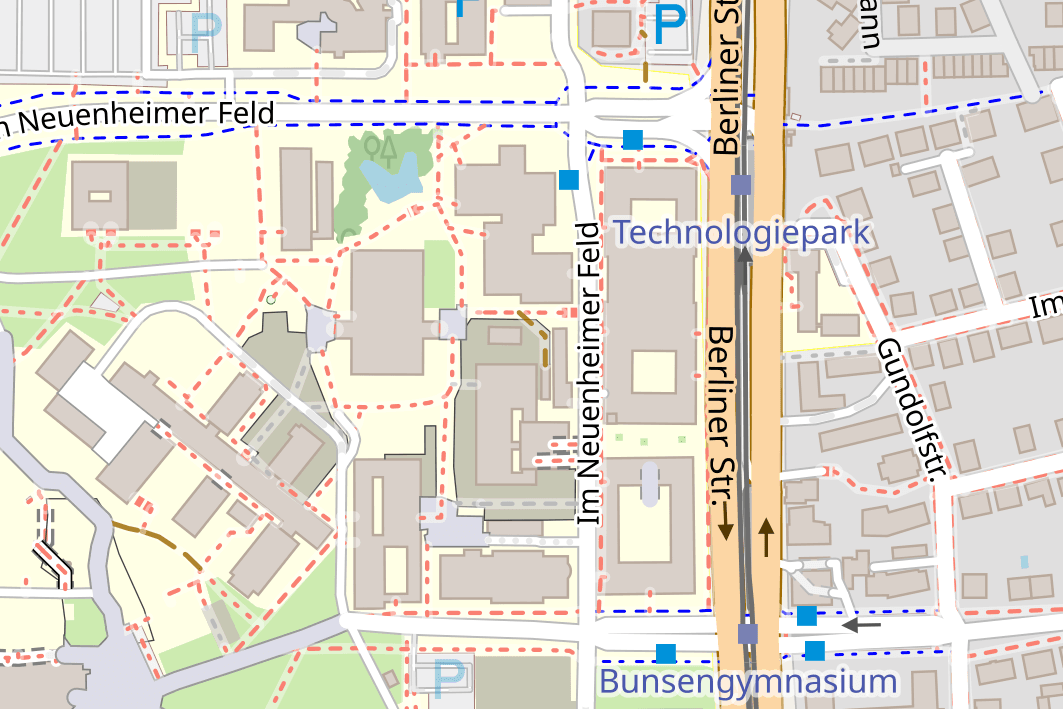
\includegraphics[height=60mm]{../templates/images/ticketkarte128-small.png}};
    \node at (34, 32) [anchor=south] {
\includegraphics[]{../templates/images/marker.png}};
    \node at (0,0) [anchor=south west, fill=white] {\tiny © OpenStreetMap contributors};
  \end{tikzpicture}
\end{minipage}
\fcolorbox{black}{white}{%
  \begin{minipage}[c][57mm][t]{0.42\linewidth}
    \RaggedRight
    \bilingualHeading{\large Location}{Veranstaltungsort}\\
    Universität Heidelberg\\
    Hörsaalzentrum Chemie\\
    Im Neuenheimer Feld 252\\
    69120 Heidelberg
  
    \largeSpace
    \bilingualHeading{\large Next tram stop}{Nächste Haltestelle}\\
    Technologiepark
  
    \largeSpace
    \bilingualHeading{\large Social Event}{Abendveranstaltung}\\
    HebelHalle, Hebelstr. 9, 69115 Heidelberg
  \end{minipage}
}
\justifying

{\small \textbf{This ticket is only valid if it is printed out and in conjunction with a valid passport or ID card.} It entitles you to travel with all buses, trams and all permitted trains (DB: RE, RB, S-Bahn, each 2nd class only) in the area of Verkehrsverbund Rhein-Neckar (VRN) in the validity period until 3:00 am on the following day. The VRN conditions of carriage and fares apply. \textbf{Do not fold the barcode.}}

\noindent\includegraphics{((( png_path)))}

\end{document}
